\section{Results}
In all the scenarios described in the previous section, the results were obtained using a PDDL planner implemented in Julia. 
Specifically, the A$*$ search algorithm was implemented. The planner initializes the problem state using the initstate function and 
defines the goals using MinStepsGoal, optimizing for minimal steps to achieve the objectives, while the planning process employs an A$*$ 
planner (AStarPlanner) with the HAddR heuristic to guide the search.


The final path obtained for each studied case can be seen in Figure \ref{fig:fig1}, Figure \ref{fig:fig2} and Figure \ref{fig:fig3}.

The code used to execute these PDDL files, along with the generated plans, is available in the accompanying Jupyter notebook file within the attached ZIP folder.

\begin{figure}[t]
    \centering
    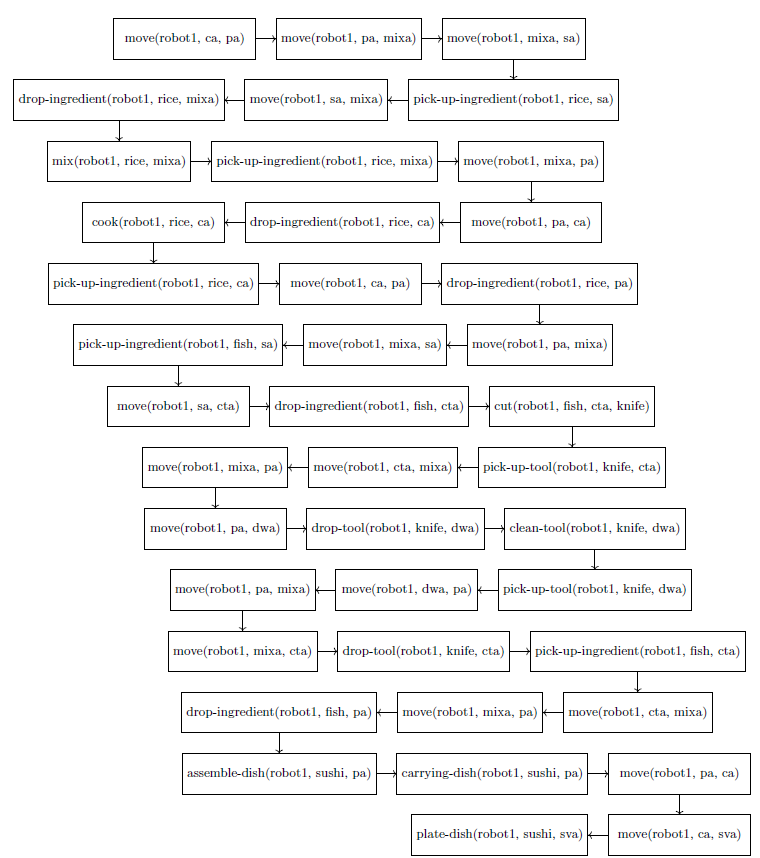
\includegraphics[width=1\linewidth]{fig1.png}
    \caption{Basic problem final solution.}
    \label{fig:fig1}
  \end{figure}

  \begin{figure}[t]
    \centering
    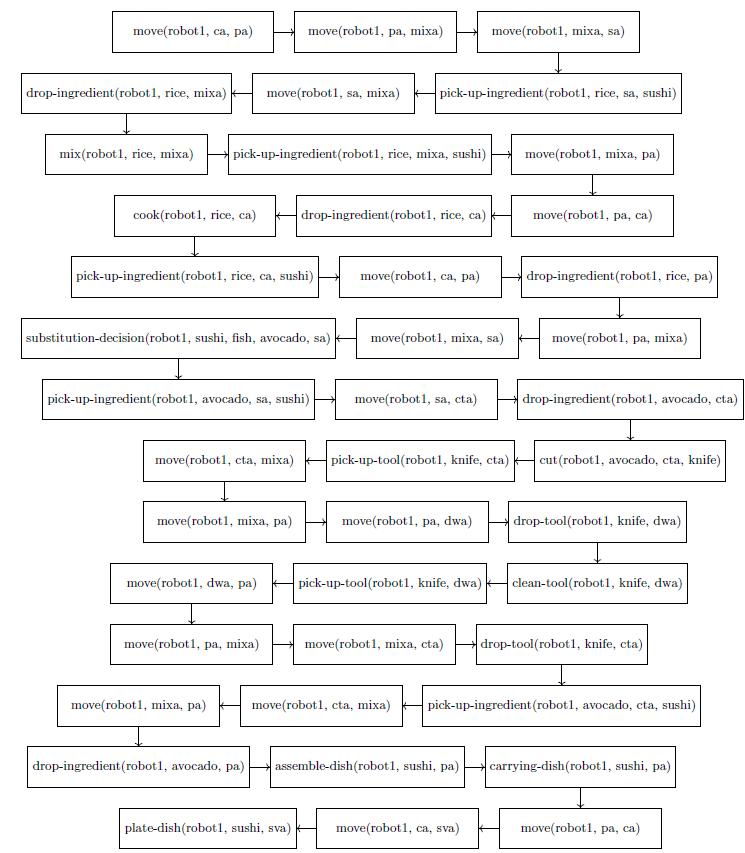
\includegraphics[width=1\linewidth]{fig2.png}
    \caption{Problem with substitution between ingredients solution.}
    \label{fig:fig2}
  \end{figure}

  \begin{figure}[h]
    \centering
    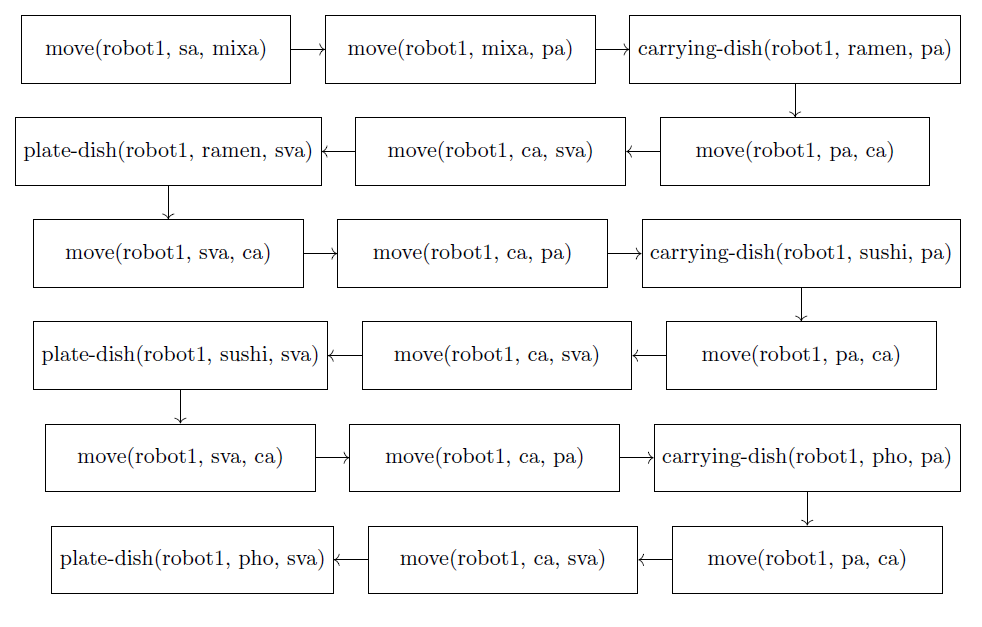
\includegraphics[width=0.7\linewidth]{fig3.png}
    \caption{Problem of priorization dishes solution.}
    \label{fig:fig3}
  \end{figure}